
\usepackage[T1]{fontenc}
\usepackage{mathptmx}
\usepackage[scaled=.90]{helvet}
\usepackage{courier}

\usepackage{beamerthemesplit}
\usepackage{verbatim}
\usepackage{hyperref}
\usepackage{listings}
\lstset{language=Perl,basicstyle=\footnotesize,tabsize=3,showstringspaces=false}

\title{Modern PerlCommerce}
\author[racke]{Stefan Hornburg (Racke)\\ \texttt{racke@linuxia.de}}
\date[]{Pittsburgh Perl Workshop, 8th October 2011}

\begin{document}
\maketitle{}

\begin{frame}
  \titlepage
\end{frame}

\tableofcontents

% \section{History}
% \begin{frame}{History}
% \begin{itemize}
% \item 1995 CGI
% \item 1995 MiniVend
% \end{itemize}
% \end{frame}

\section{Modern PerlCommerce}
The theme of this conference is ``Modern Perl''.

\subsection{* Perl}
There is a lot of talk about marketing Perl, modern Perl
and even postmodern Perl.

\begin{frame}{* Perl}
\begin{itemize}
\item Marketing Perl
\item Modern Perl
\item Postmodern Perl
\end{itemize}
\end{frame}

That sounds wonderful, but what does that really mean for Ecommerce
projects?

\subsection{Modern Perl}
There isn't really a set definition what Modern Perl is about,
but I want to point the things important to us.

\begin{frame}{Modern Perl}
\begin{itemize}
\item CPAN
\item Best Practices
\item Tests
\item Separation (Modules, Plugins, Hooks, Templates)
\item PSGI/Plack
\end{itemize}
\end{frame}

\subsection{PerlCommerce Choices}
Surprisingly there are not many choices for OpenSource PerlCommerce
software. Searching for ``cart'', ``ecommerce'' or ``shop'' on CPAN
gives you only a few results, which aren't actually very helpful.

Let's look at the possible choices for OpenSource PerlCommerce software:

\begin{frame}{PerlCommerce Choices}
\begin{itemize}
\item Interchange
\item Handel
\item Agora
\item Business::Cart::Generic
\end{itemize}
\end{frame}

Interchange is around since 1995, but not in CPAN.

Handel is a framework which support AxKit, Template Toolkit 
and Catalyst.
Available from CPAN, last release a year ago.
There isn't even a mailing list.

Agora isn't modern Perl either and is around since 1999.

Business::Cart::Generic claims to be a basic shopping cart,
the synopsis says Convert parts of osCommerce and PrestaShop into
Perl.

% solid +
% fast +
% archaic -
% monolithic -

\begin{frame}{Status quo}
  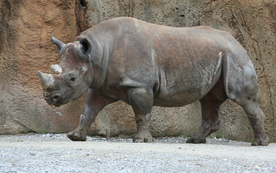
\includegraphics{rhino.jpg}
\end{frame}

\begin{frame}{Future}
  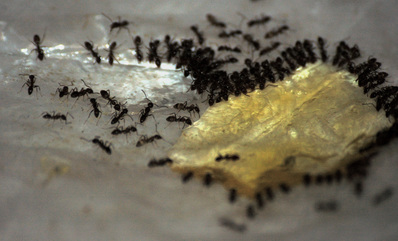
\includegraphics{ants.jpg}
\end{frame}

\subsection{References}
\begin{frame}{References}
\begin{itemize}
\item Backcountry \url{http://www.backcountry.com/}
\item Fragnance \url{http://www.fragrancenet.com/}
\item DoS \url{https://vsc.state.gov/}
\end{itemize}
\end{frame}

\subsection{Dancer Offerings}
\begin{frame}{Dancer Offerings}
Things supplied by Dancer or Dancer plugins:

\begin{itemize}
\item Dispatching requests
\item Session handling
\item Template engine
\item I18N
\end{itemize}
\end{frame}

\subsection{How easy can it be?}
\begin{frame}[fragile]{How easy can it be?}
\begin{lstlisting}
#!/usr/bin/env perl

use Dancer;
use Dancer::Plugin::Interchange;

sell;
\end{lstlisting}
\end{frame}

\subsection{Real World}
Running and maintaining an online shop is a challenging business
and requires constant change to stay on top of your competitors.

\begin{frame}{Real World}
\begin{itemize}
\item Marketing, SEO
\item Legal stuff
\item Interfaces
\item Design
\end{itemize}
\end{frame}

\section{API}
\subsection{Cart}
\begin{frame}{Cart}
\begin{itemize}
\item SKU, Name, Quantity, Price
\item Price > 0
\item Combines automatically
\item Multiple carts
\item Storage everywhere
\end{itemize}
\end{frame}

\begin{frame}[fragile]{Nitesi::Cart Functions}
\begin{lstlisting}
$cart = Nitesi::Cart->new;

$cart->add(sku => 'POM253', name => 'Pomelo',
    price => 3.00, quantity => 10);

$cart->remove(sku => 'POM253');

$cart->count();

$cart->clear();

$cart->total();

$cart->subtotal();
\end{lstlisting}
\end{frame}

\subsubsection{Everything is a Cart}
\begin{frame}{Everything is a Cart}
\begin{itemize}
\item Saved Carts
\item Wishlists
\item Collections
\end{itemize}
\end{frame}

\subsubsection{Cart Backends}
\begin{frame}{Cart Backends}
\begin{itemize}
\item Session
\item DBI
\end{itemize}
\end{frame}

\subsubsection{Inventory Checks}
Inventory checks are pretty much limited in Interchange right now.
They are controlled by the configuration directives MinQuantityField
and MaxQuantityField:
\begin{frame}[fragile]{Inventory Check}
\begin{lstlisting}
MinQuantityField min_quantity
MaxQuantityField inventory:quantity 
\end{lstlisting}
\end{frame}
Also they are part of the standard code instead of loaded through
hooks.

\subsection{Payment}
\begin{frame}{Payment}
\begin{itemize}
\item Business::OnlinePayment
\end{itemize}
\end{frame}

\subsection{Taxes}
Tax on top of the product cost can be applied in different varieties.

Germany has 19\% salestax, 7.5\% reduced salestax for books and some
items are tax free. You have to show the breakdown of different taxes
on the receipt.

Orders for businesses between different countries of the EU are exempt
of salestax if the buying party has a salestaxid.

\begin{frame}{Taxes}
\end{frame}

Business::Tax::VAT doesn't account for reduced rates.

\begin{frame}{Tax Modules on CPAN}
\begin{itemize}
\item Business::Tax::Canada
\item Business::CA::GST
\item Business::Tax::VAT
\item Business::Tax::VAT::Validation
\end{itemize}
\end{frame}

\subsection{Shipping}
\begin{frame}{Shipping}
\begin{itemize}
\item Simple Shipping
\item Crazy Shipping
\item Shipping API
\end{itemize}
\end{frame}

\subsection{Account Management}
\begin{frame}{Account Management}
\begin{itemize}
\item Customer Service
\item Menus
\item Backend
\end{itemize}
\end{frame}

\begin{frame}{Account manager}
\begin{itemize}
\item Account Providers
\item Login/Logout
\item Login status
\item Account Information
\end{itemize}

\end{frame}
\subsection{Access Control}
\begin{frame}{Access Control}
\begin{itemize}
\item User
\item Roles
\item Permissions
\end{itemize}
\end{frame}

\subsection{Forms}
\begin{frame}{Forms}
\begin{itemize}
\item Display
\item Validation
\item Storage
\end{itemize}
\end{frame}

\subsection{PDF Invoices}
\begin{frame}{PDF Invoices}
\begin{itemize}
\item HTML template
\item Template::Flute::PDF
\end{itemize}
\end{frame}

\subsection{Backend}
\begin{frame}{Shipping}
\end{frame}

\section{Integration \& Deployment}
\subsection{Dancer}
\subsubsection{Routes}
\begin{frame}{Routes}
\begin{itemize}
\item Categories
\item Products
\item Cart
\item Checkout
\item Customer Service
\end{itemize}
\end{frame}

\subsubsection{Default Route}
Categories and products can be handled through the default route
(see
\url{http://search.cpan.org/~sukria/Dancer/lib/Dancer/Cookbook.pod#Default_route})
as alternative to defining explicit routes.

\begin{frame}[fragile]{Default Route}
\begin{lstlisting}
get qr{/(.*)} => sub {
    my ($sku) = splat;
    my $product;

    # check for existing product
    if ($product = database->quick_select('products', {sku => $sku})) {
        # display flypage
        template 'flypage', $product;
    }
    else {
        # display not found page
        status 'not_found';
        forward '404';
    }
};
\end{lstlisting}
\end{frame}
\end{document}

%%% Local Variables: 
%%% mode: latex
%%% TeX-master: t
%%% End: 
